\section{Ablauf}
\label{sec:ablauf}

Im Folgenden wird der Ablauf beschrieben, den \textit{Silisloth} beim Absolvieren der gestellten Wettbewerbsaufgabe befolgt:

\begin{description}
    \item[Vorbereitung] \textit{Silisloth} wird hinten am Seil montiert und in Ausgangsposition gebracht. Der Raspi ist mit dem eigens über einen Access-Point zur Verfügung gestellten WiFi-Netzwerk \texttt{pren7} verbunden. Der Arduino ist per USB-Kabel an den Raspi angeschlossen. Der Raspi wird über eine USV von einem LiPo-Akku gespeist. Die Motoren, Pumpen und das Ventil werden über einen weiteren LiPo-Akku mit Strom versorgt. Die Smartphone-App (\secref{sec:smartphoneapp}) ist auf einem Smartphone geöffnet. Auf einem Laptop, der per \texttt{ssh} über das WiFi-Netzwerk mit dem Raspi verbunden ist, kann die Raspi-Anwendung (\secref{sec:raspi}) gestartet werden, sodass der darin enthaltene TCP-Server auf das vom Smartphone aus erteilte Startsignal wartet. Beim Start der Raspi-Anwendung werden weiter die Ultraschallsensoren initialisiert und die serielle Verbindung zum Arduino erstellt. Auf dem Arduino läuft ebenfalls ein Programm (\secref{sec:arduino}), das auf Befehle vom Raspi hört (\secref{sec:kommunikation}).
    \item[Erteilung Startsignal] Nachdem das Startsignal mündlich erteilt worden ist («drei, zwei, eins, Start»), wird die \textit{Start}-Schaltfläche auf der Smartphone-App betätigt. Das Smartphone nimmt die Verbindung zum TCP-Server auf dem Raspi auf und erteilt diesem das Startsignal.
    \item[Zur Last fahren] Der Raspi erteilt dem Arduino den Befehl zum Losfahren (\texttt{G} wie «go»). Da die Last zu Beginn an einer genau definierten Position vor dem Anfangspfosten liegt, und da der Abstand vom Anfangs- zum Endpfosten bekannt und konstant ist, kann die Position über der Last mit dem nach vorne zeigenden Ultraschallsensor (X-Ultraschallsensor) ermittelt werden. Der Getriebemotor läuft so lange, bis die zuvor berechnete Distanz zwischen X-Ultraschallsensor und Endpfosten erreicht ist. (Der Abstand zwischen X-Ultraschallsensor und Mittelpunkt des Silikongreifers ist miteinberechnet.)
    \item[Die Last greifen] Ist nun der Silikongreifer über der Last platziert, muss \textit{Silisloth} anhalten und den Greifer herunterlassen. Dazu wird mit dem Ultraschallsensor, der nach unten zeigt (Z\hyp{Ul\-tra\-schall\-sen\-sor}), die Distanz zum Boden gemessen. Der Raspi erteilt dem Arduino nun den Befehl \texttt{Sxxx;}, wobei \texttt{S} für «stop» steht und \texttt{xxx} für die Anzahl Millimeter (terminiert mit Semikolon), die der Z-Ultraschallsensor als Abstand über dem Boden ermittelt hat. Der Abstand zwischen Z-Ultraschallsensor und Greifer wird herausgerechnet, und die von der Greifereinheit zurückzulegende Distanz wird in Schritte für den Stepper-Motor umgerechnet. Ist die Greifereinheit auf der Last positioniert, wird der Silikongreifer mit den beiden Luftpumpen aufgepumpt, sodass er sich ausdehnt und die Last möglichst eng umschliesst. Die Ventile werden anschliessend geschlossen.
    \item[Weiterfahren] Die Greifeinheit wird um die gleiche Distanz angehoben, wie sie zuvor heruntergelassen wurde. Ist dies abgeschlossen, schickt der Arduino dem Raspi ein entsprechendes Signal (\texttt{L} für «Last bereit»). Von nun an wird der Abstand der Last zum Boden mittels Ultraschallmessungen (Z-Ultraschallsensor) ermittelt, wovon der Abstand zwischen vertikalem Lastmittelpunkt und Z-Ultraschallsensor jeweils von der ermittelten Höhe subtrahiert wird. Der Abstand zum Endpfosten wird über den X-Ultraschallsensor ermittelt; X- und Z-Koordinaten werden auf das Smartphone übertragen. \textit{Silisloth} fährt mit erhöhtem Tempo weiter.
    \item[Zielfeld entdecken] Nachdem der Raspi erkannt hat, dass die Fahrt wieder aufgenommen wurde, wird die Bildverarbeitung aktiviert. Sobald das Zielfeld zum ersten Mal «erkannt» wurde, wird die Fahrtgeschwindigkeit reduziert, wozu der Raspi dem Arduino den Befehl zum Verlangsamen (\texttt{D} für «decelerate») schickt. Die Fahrtgeschwindigkeit wird reduziert, damit die Zielfelderkennung mehr Bilder pro Zeiteinheit verarbeiten und so die Endposition genauer bestimmen kann.
    \item[Zielposition bestimmen] In verlangsamter Fahrt werden nun weitere Bilder vom Zielfeld aufgenommen und ausgewertet. Sobald die Zielfelderkennung eine horizontale Distanz von unter $15cm$ zum Mittelpunkt des Zielfeldes ausgemacht hat, wird die weitere Positionierung mit dem X-Ultraschallsensor vorgenommen. (Da die Kamera vorne angebracht ist, kann sie das Zielfeld nicht mehr «sehen», sobald die Last darüber positioniert ist, da die Greifeinheit den Blick darauf versperrt.) Die beiden zuletzt ermittelten Distanzen -- optisch und per Ultraschallsensor -- werden zwischengespeichert. Aus diesen Angaben kann nun die Distanz berechnet werden, die der X-Ultraschallsensor zum Endpfosten haben muss, um die Last in der Mitte des Zielfeldes abzuwerfen (siehe dazu \calcrefplain{eq:enddistanz} und \imgrefplain{fig:enddistanz}).
    \item[Last abwerfen] Sobald die vom X-Ultraschallsensor gemessene Distanz kleiner oder gleich der zuvor ermittelten Enddistanz ist, kann die Last abgeworfen werden. Hierzu verwendet der Raspi wiederum den Befehl der Form \texttt{Sxxx;}, um die Greifeinheit um die vom Z-Ultraschallsensor ermittelte Anzahl Millimeter zum Boden herunterzulassen. Der Greifer wird über die Ventile gelöst -- was wesentlich schneller geht, als das Aufpumpen -- und die Last wird möglichst genau in der Mitte des Zielfeldes liegen gelassen. Die Übertragung der X- und Z-Koordinaten wird nun eingestellt, wobei die Z-Koordinaten beim Absetzen der Last berechnet und nicht gemessen werden.
    \item[Zum Endpfosten fahren] Der Arduino teilt dem Raspi über das \texttt{L}-Signal («Last bereit») mit, dass die Fahrt nun wieder aufgenommen wird. Dies geschieht zunächst mit voller Geschwindigkeit, bis der X-Ultraschallsensor eine Distanz von weniger als $25cm$ meldet. Die Geschwindigkeit wird reduziert, indem der Raspi das \texttt{D}-Signal («decelerate») an den Arduino schickt. Der Endtaster ist ca. $15cm$ vor dem X-Ultraschallsensor angebracht, sodass die letzten $10cm$ in langsamer Fahrt zurückgelegt werden. Bei der Berührung mit dem Endpfosten wird der Mikroendschalter betätigt, was vom Raspi registriert wird. Er erteilt nun das \texttt{H}-Signal (für «halt») an den Arduino, damit dieser den Motor stoppen kann.
    \item[Zurückfahren] Nach wenigen Sekunden am Endpfosten fährt \textit{Silisloth} automatisch einige Sekunden zurück, sodass ein weiterer Durchlauf in Angriff genommen werden kann.
\end{description}

\subsection{Berechnung der Enddistanz}

\begin{align}
    E_{\overline{XP}} &= D_{\overline{XP}}-D_{\overline{KZ}}-D_{\overline{KX}}-D_{\overline{KL}} \label{eq:enddistanz} \\
    E_{\overline{XP}} &= \text{Enddistanz von X-Ultraschallsensor zum Endpfosten} \nonumber \\
    D_{\overline{XP}} &= \text{aktuelle Distanz von X-Ultraschallsensor zu Endpfosten} \nonumber \\
    D_{\overline{KZ}} &= \text{aktuelle Distanz von Kamera zu Zielfeldmittelpunkt} \nonumber \\
    D_{\overline{KX}} &= \text{Abstand von Kamera zu X-Ultraschallsensor und} \nonumber \\
    D_{\overline{KL}} &= \text{Abstand von Kamera zu Lastmittelpunkt} \nonumber
\end{align}

\begin{figure}[H]
    \centering
    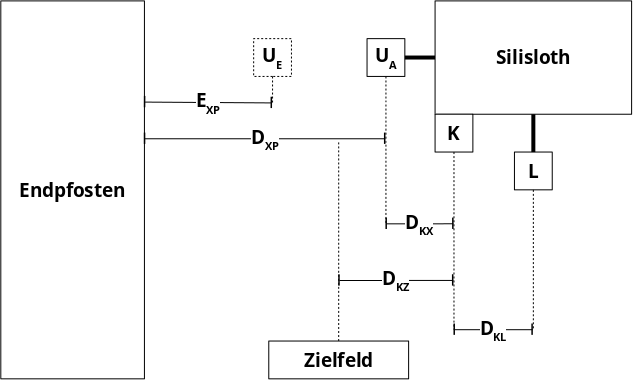
\includegraphics[width=0.8\textwidth]{graphs/enddistanz.png}
    \caption{Die Berechnung der Enddistanz (Position des Lastabwurfs): Der Ultraschallsensor muss von Position $U_{A}$ nach $U_{E}$ gebracht werden, sodass er eine Distanz von $E_{\overline{XP}}$ bis zum Endpfosten misst, und sich die Last über der Mitte des Zielfelds befindet.}
    \label{fig:enddistanz}
\end{figure}

